\documentclass[handout]{beamer}

\usepackage{fontspec} 
\useoutertheme{lsp}

\usepackage{lsptitle}

\def\two@digits#1{\ifnum#1<10 0\fi\number#1}
\def\mytoday{\two@digits{\number\day}.\two@digits{\number\month}.\number\year}


\usepackage{xspace,multicol}
\newcommand{\latex}{\LaTeX\xspace}
\usepackage{tikz}

\usepackage{avm,forest}

\newcounter{lastpagemainpart}
\footnotesep0pt
\renewcommand{\footnoterule}{}
\usefootnotetemplate{
  \noindent
  \insertfootnotemark\insertfootnotetext}

\let\beamerfn=\footnote
\renewcommand{\footnote}[1]{%
\let\oldfnsize=\footnotesize%
\let\footnotesize=\tiny%
\beamerfn<\thebeamerpauses->{#1}%
\let\footnotesize=\oldfnsize}


\date[20.11.2014]{\mbox{20.11.2014  MPI für Wissenschaftsgeschichte, Berlin}}

\usepackage{eurosym}  
 
\renewcommand{\centerline}[1]{\hfill#1\hfill\hfill\mbox{}}


\title{\mbox{Language Science Press}}
% \institute{FU Berlin}
\author[Nordhoff]{Sebastian Nordhoff}



\begin{document}
\lspbeamertitle

\section{Einleitung}

\frame{
\frametitle{Language Science Press}
\begin{itemize}
\item Open-Access-Publikationen
\item Publikation sprachwissenschaftlicher Monographien
\item Spitzenforschung
\item Reihenbasiert
\item Communitybasiert 
\end{itemize}

\begin{itemize}
 \item http://www.langsci-press.org
\end{itemize}

}


\frame{
\frametitle{Geschichte}
\begin{itemize}
\item Juni 2012 erstes Treffen mit Adele Goldberg, Thomas Herbst, Anatol Stefanowitsch
\item August 2012 OALI-Webseite, Mails an prominente Kollegen
\begin{itemize}
 \item ehemaliger Name: Open Access in Linguistics
\end{itemize}
\item Oktober 2012 Kick-Off-Treffen an der FU-Berlin mit internationaler Beteiligung via Skype  
\item Februar 2013 Einreichung Antrag im DFG-Programm \emph{Wissenschaftliche Monographien und monographische Serien im Open Access}
\item Dezember 2013 DFG-Finanzierungszusage, 2 von 17 Projekten gefördert, $>$~575,000 € für zwei Jahre,
  72\,\% der Gesamtfördersumme  
\end{itemize}
}

\frame{
\frametitle{Geschichte}
\begin{itemize}
\item Februar 2014 Einstellung Koordinator
\item März 2014 Publikation der ersten Bücher
\item Juni 2014 Einstellung weiterer Mitarbeiter
\item November 2014 57 Anfragen, 18 angenommene Bücher, 4 veröffentlichte Bücher
\end{itemize}
}

\frame{
\frametitle{Katalog}
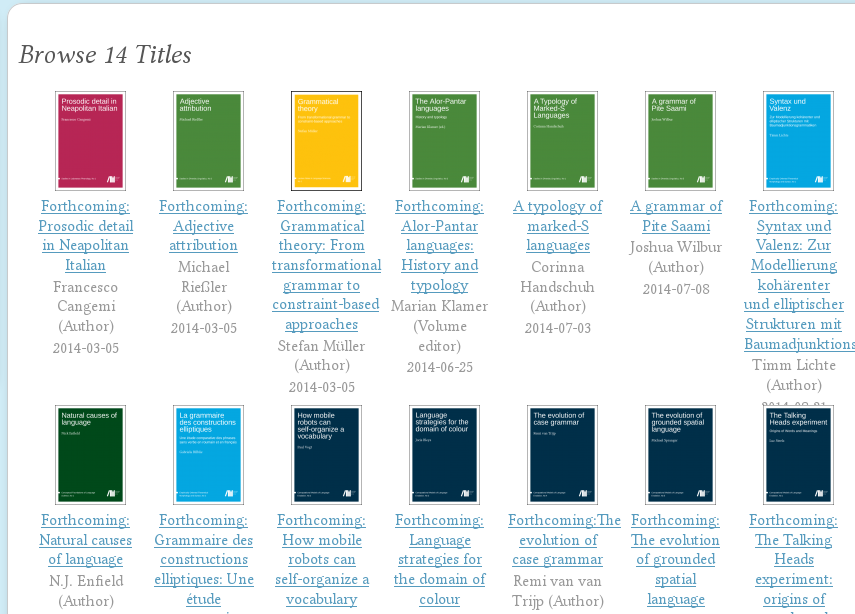
\includegraphics[width=.95\textwidth]{pics/catalog.png}
}


% 
% \frame{
% \frametitle{Personal}
% \begin{itemize}
% \item Frontend-Entwickler
%   \begin{itemize}
%   \item     Gamification
%   \item     Open Review
%   \end{itemize}
% \item Sys-Admin
% \item \LaTeX-Entwickler
% \item Koordinator
% \item Controllerin
% \end{itemize}
% }


\frame{
\frametitle{Sprachwissenschaft}

\begin{columns}
 \begin{column}{6cm}
\begin{itemize}
\item Im Vergleich zu anderen Geisteswissenschaften recht computeraffin
\begin{itemize}
 \item Schnittstelle Computerlinguistik
 \item Formalismen
 \item quantitative Methoden
\end{itemize}
\item Open Access auch durch Kontakt mit ärmeren Weltregionen relevant
\end{itemize}  
 \end{column}
 \begin{column}{4cm}
 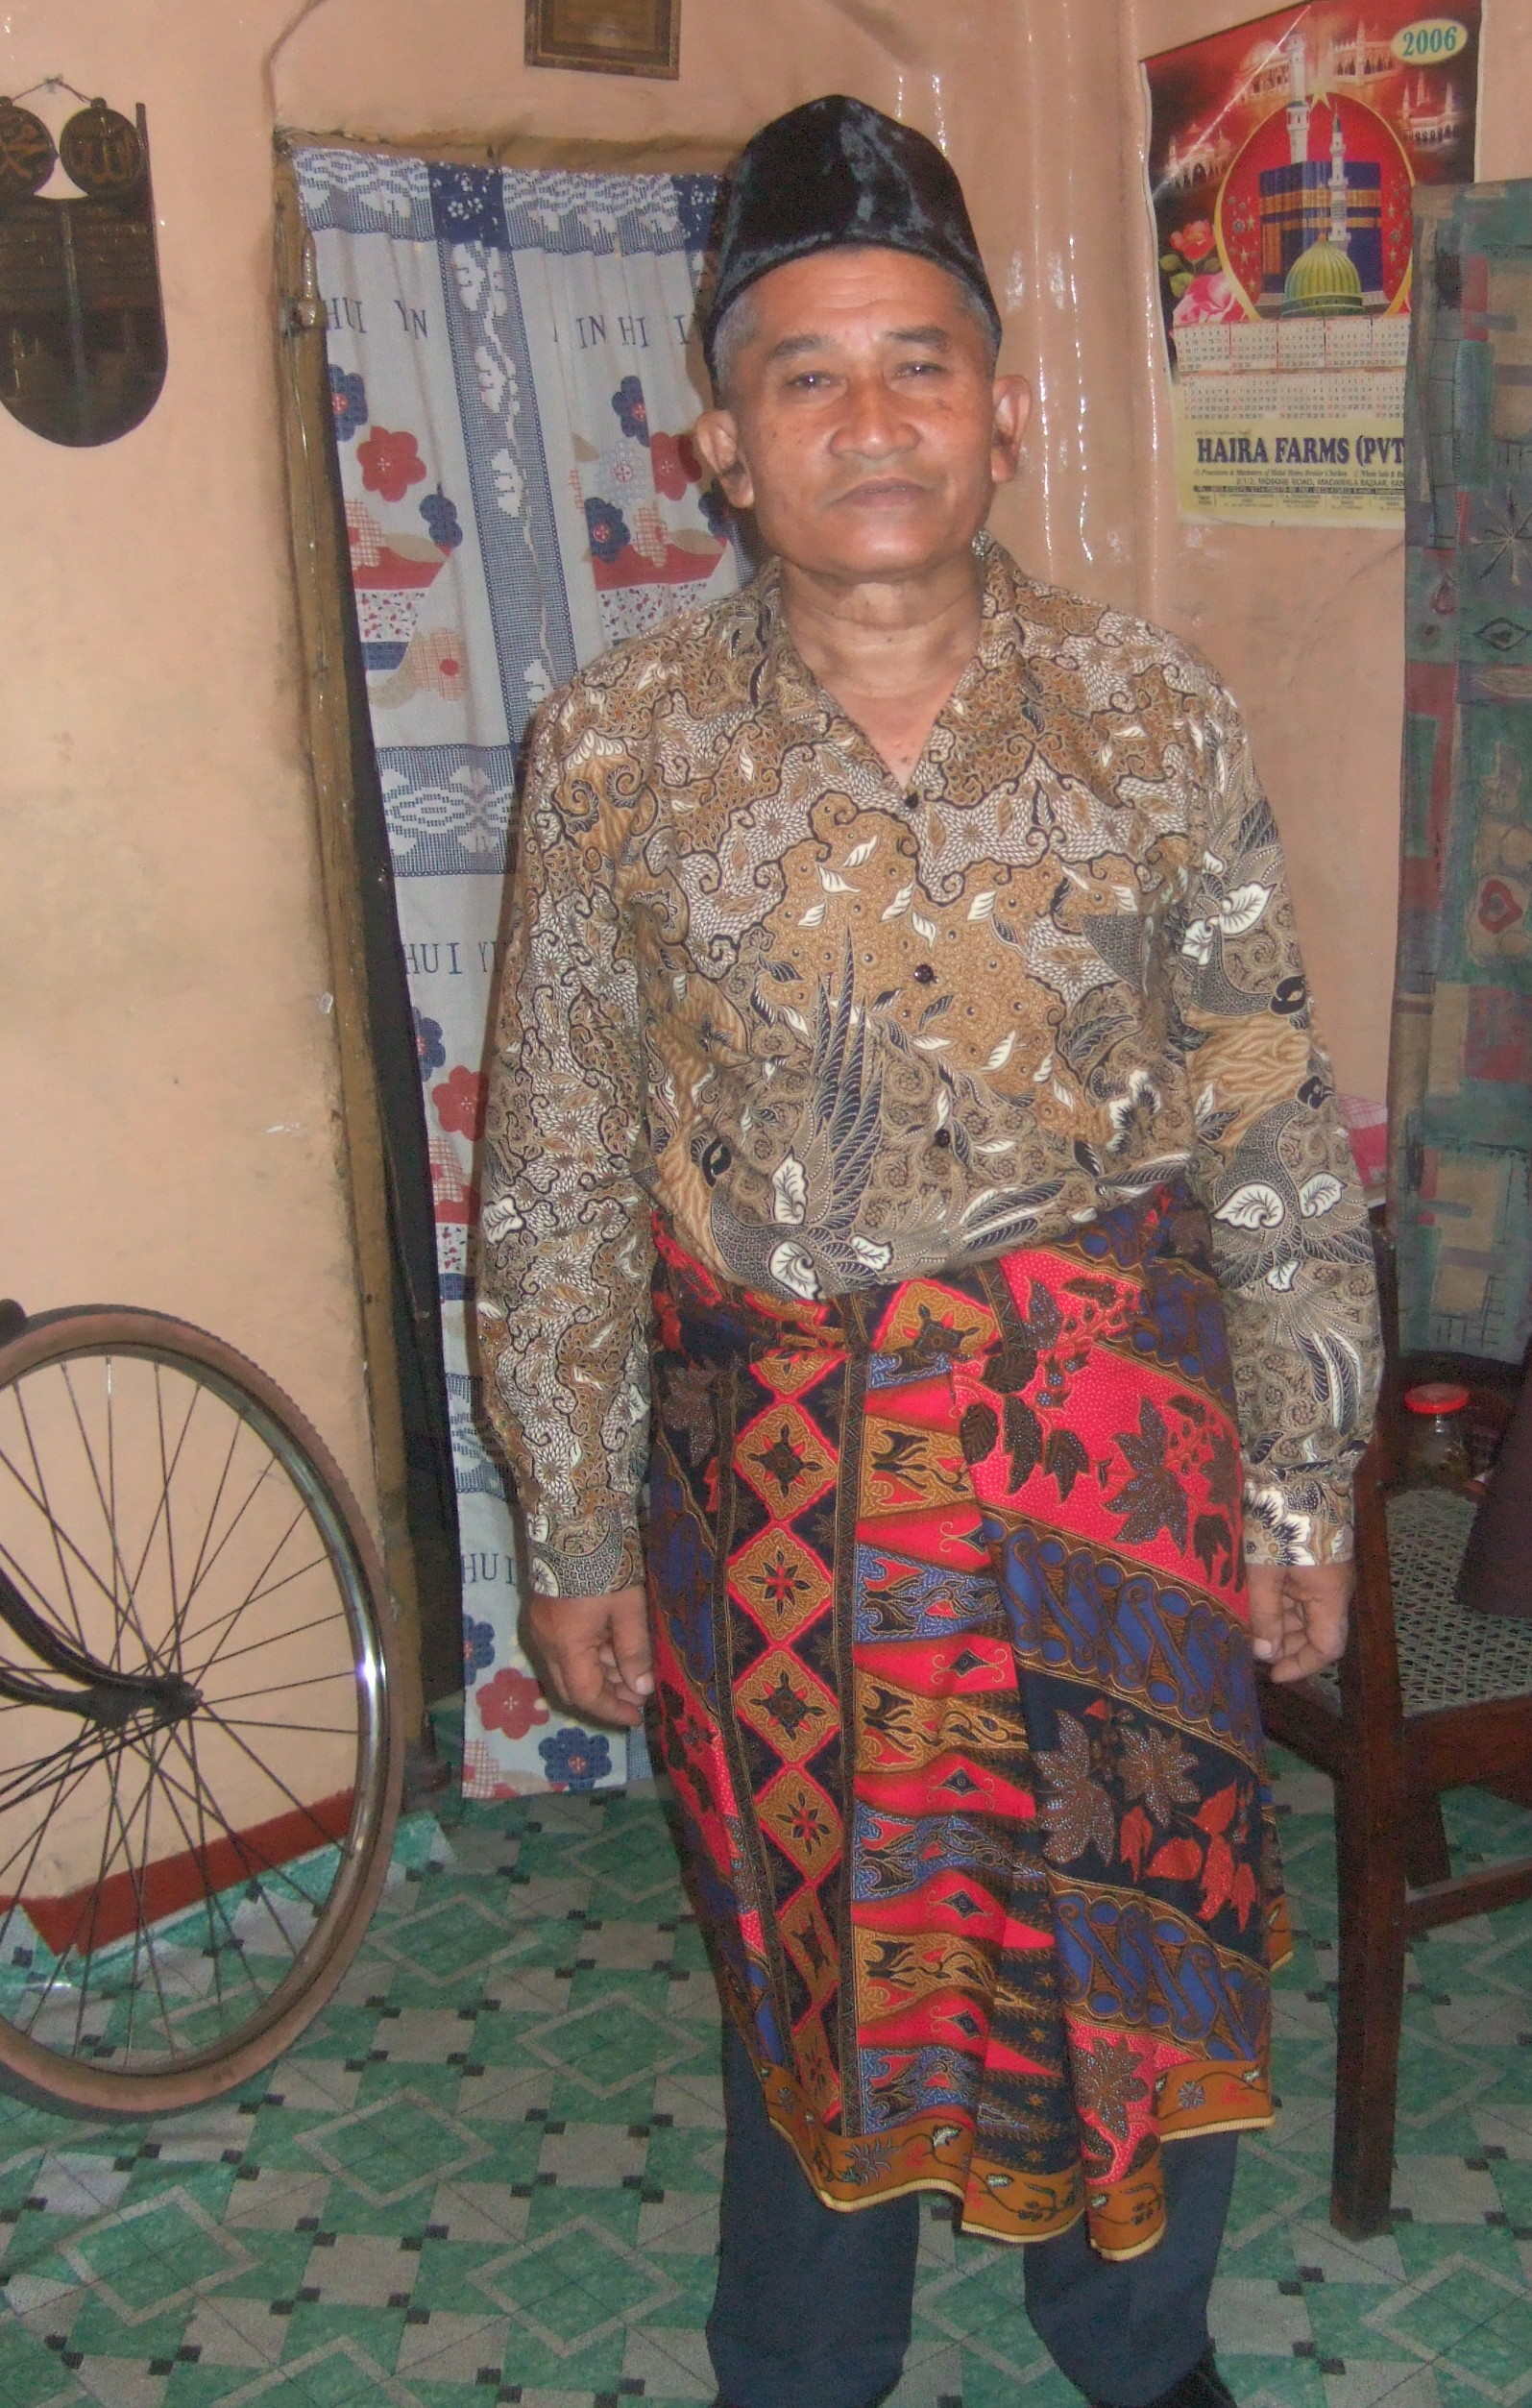
\includegraphics[width=4cm]{pics/cassiere.jpg} %GDP nominal $3,385/yr in Sri Lanka = 2613 EUR. 217 EUR per month 
 \end{column}
\end{columns}
}


            
\section{Prinzipien}

\frame{
\frametitle{\raggedright Prinzipien von \mbox{Language~~~~~} \mbox{Science} Press}
\begin{enumerate}
 \item      Prestige
 \begin{itemize}
  \item         soviel Prestige wie möglich in sowenig Zeit wie möglich
  \item         Champions League      
 \end{itemize}              
 \item      Rückhalt in der Community
 \begin{itemize}
  \item  Communitybuilding
  \item  Jedes Buch muss in einer Reihe erscheinen
  \item  Reihenherausgeber organisieren selbständig
  \item Adivsory Board evaluiert Reihen
 \end{itemize}
 \item      betriebswirtschaftliche Fundiertheit       
\end{enumerate}
 
}
% 
% \frame{
% \frametitle{ Platinum OA}
% \begin{itemize}
% \item  Platinum OA
% \end{itemize}
% }

\section{Umsetzung}
\subsection{Prestige}
\frame{
\frametitle{Prestige}
\begin{itemize}
\item Motivationsgefüge der Autoren berücksichtigen
\begin{itemize}
 \item Karma $\Longleftrightarrow$ Karrierechancen
\end{itemize}
\item Karrierechancen sind ein wesentlicher Faktor bei der Wahl eines Verlages 
\item Open Access kann nur dann Bestand haben, wenn die Karrierechancen nicht darunter leiden
\item Karrierechancen korrelieren mit Prestige der Veröffentlichungsorte
\item $\to$ ein neuer Verlag muss sehr schnell sehr viel Prestige aufbauen
\end{itemize}
}

\frame{
\frametitle{Quellen von Prestige}
\begin{enumerate}
 \item Prominente Unterstützer
 \item Menge an Unterstützern
 \item Qualität der Bücher
 \item Selektivität/Exklusivität
\end{enumerate}
}

\frame{
\frametitle{Prominente Unterstützer}

    \parbox{.4\textwidth}{
      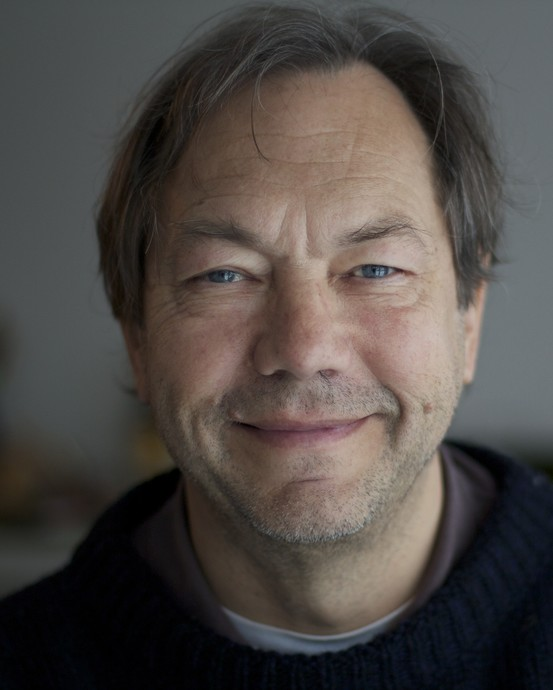
\includegraphics[height=.8\textheight]{pics/steels-s.jpg}
      
      Luc Steels
      }
    \parbox{.4\textwidth}{
      ~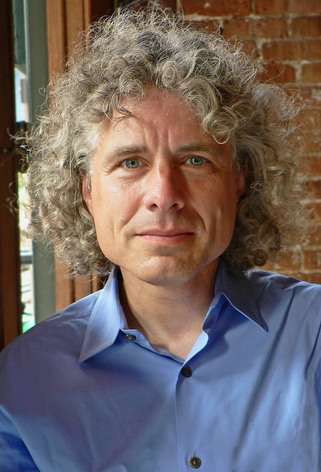
\includegraphics[height=.8\textheight]{pics/pinker-s.jpg}
      
      Steven Pinker
    }
}



\frame{
\frametitle{Menge an Unterstützern}
\begin{itemize}
\item    öffentlich einsehbare Supporterseite 
\begin{itemize}
 \item \url{http://langsci-press.org/Meta/sign/supporters}
\end{itemize}
\item    Mailingliste
\item    ``Pledge to Publish'' vor Projektstart
\item    kritische Masse war schon vor Projektstart erreicht
\item    Start auf der Jahrestagung der Deutschen Gesellschaft für Sprachwissenschaft 
mit dem ersten Buch 7 Tage nach Projektbeginn
\end{itemize}
}


\frame{
\frametitle{Formale Qualität}
\begin{itemize}
\item \LaTeX
\item Ligaturen 
\parbox{.3\textwidth}{
\includegraphics[width=.3\textwidth]{pics/affin.png}}
\end{itemize}

\begin{itemize}
\item Alleinstellungsmerkmale
\begin{itemize}
 \item  c\&p-fähiges Unicode, á statt  ´a
 \item  CI Font (Libertine)
 \item  neue Glyphen
 
\parbox{.3\textwidth}{
\includegraphics[width=.3\textwidth]{pics/schwaengma.png}}
 \end{itemize}
\end{itemize}
}

\frame{
\frametitle{Formale Qualität}
\begin{itemize}
\item Chinesisch, Hebräisch, Arabisch
\item diverse fachspezifische Erweiterungen
\item Namensindex, Sprachindex, thematischer Index
\item klickbare Querverweise
\item Print-on-Demand
\begin{itemize}
 \item theoretisch noch Prestige durch hohen Preis im dreistelligen Bereich
 \item bei Language Science Press ca. 30 EUR/Buch
\end{itemize}

\end{itemize}
}

\frame{
\frametitle{Inhaltliche Qualität}
\begin{itemize}
\item traditioneller Peer Review
\begin{itemize}
 \item organisiert vom Reihenherausgeber zusammen mit Editorial Board
\end{itemize}
\item keine Dissertationen (Selektivität)
\item Commitment
\begin{itemize}
 \item innerhalb von 3 Monaten Annahme oder Ablehnung
 \begin{itemize}
  \item kein ``Major Revisions'' oder ``Revise and Resubmit''
 \end{itemize}
 \item innerhalb von 9 Monaten Veröffentlichung
\end{itemize}
\end{itemize}


\parbox{10cm}{\begin{flushright}
%              
\includegraphics[height=.4\textheight]{pics/approved.jpg} 
             \end{flushright}
             }
}

\subsection[Rückhalt]{Rückhalt in der Community}
\frame{
\frametitle{Einbindung der Community}

\begin{columns}
 \begin{column}{5cm}
\begin{itemize}
  \item supporter: $>$500
  \begin{itemize}
  \item 159 Prof., 239 Dr.
  \end{itemize}
  \item reader: 286
  \item reviewer: 276
  \item series editor: 24
\end{itemize}  
 \end{column}
 \begin{column}{5cm}  
\begin{itemize}  
  \item proofreader: 80 (15)
  \item typesetter: 32 (6)
  \item Font-Designer: 1
  \item Grafik-Designer: 1
  \item Latex-Guru: 1      
  \end{itemize}
 \end{column}
\end{columns}

\begin{itemize}
 \item Entwicklung eines Gamification-Plugins für Open Monograph Press 
 \item Verstetigung des Communitybeitrags
\end{itemize}


}



\frame{
\frametitle{Statistik}

\begin{columns}
\begin{column}{6cm}
\begin{itemize}
\item Reihen:
  \begin{itemize}
   \item     Bei Antragstellung projiziert   
   \begin{itemize}
    \item 2014: 5 2015:7 2016:9
   \end{itemize}
    \item            Bei Start 9
    \item           Jetzt 14
  \end{itemize}
\item Bücher:
   \begin{itemize}
    \item   57 Anfragen
    \item   18 akzeptiert (in 6 Reihen)
    \item    4 veröffentlicht
    \item    11 abgelehnt        
   \end{itemize}
\end{itemize}
\end{column}
\begin{column}{4cm}
 \parbox{4cm}{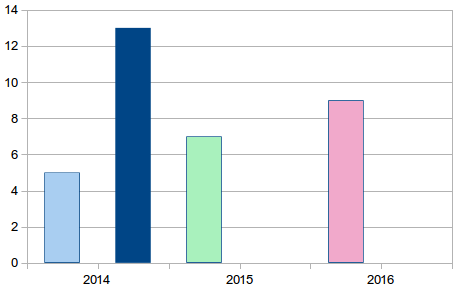
\includegraphics[width=4cm]{pics/reihen.png}\vspace{2cm}}
\end{column}
\end{columns}

}


\subsection[BWL]{Betriebswirtschaftliche Fundiertheit}

\frame{
\frametitle{Betriebswirtschaftliche Fundiertheit}
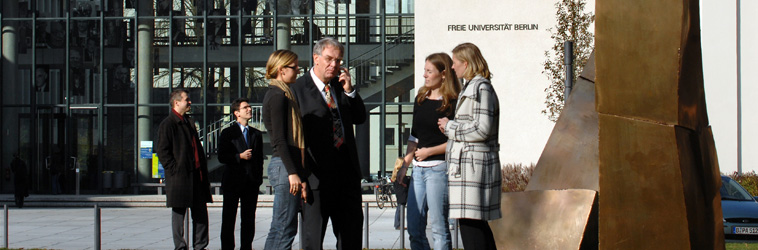
\includegraphics[width=\textwidth]{pics/slides_4spalten_1.jpg}
}



\frame{
\frametitle{Betriebswirtschaftliche Fundiertheit}
\begin{itemize}
\item Zusammenarbeit mit dem Lehrstuhl für Wirtschaftsinformatik der FU
\item Studentischer Businessplan liegt vor, wird in Teilen in eigentlichen Businessplan übernommen
\item proaktive Gestaltung der Dienstleistungslandschaft
    \begin{itemize}
    \item Print-on-Demand-Service
    
    \parbox{7cm}{
    
\includegraphics[width=2cm]{pics/epubli.png}
    \hspace{1cm}
    
\includegraphics[width=1cm]{pics/1buch.jpg}
    \hspace{1cm}
    
\includegraphics[width=1cm]{pics/bod.png}
    }
    
    \item Konversionsdienstleister doc2tex 
    
    \parbox{2cm}{
\includegraphics[width=1cm]{pics/cidleslogo.png}}
    \item Dienstleistungslandschaft auf jeden Fall nachnutzbar durch andere Projekte
    \end{itemize}
\end{itemize}
}

\frame{
\frametitle{Kosten}
\begin{columns}
 \begin{column}{5cm}

\begin{itemize}
\item Kostenarten
\begin{itemize}
 \item Personal
 \item Sachmittel
 \item Reise
 \item PR
 \item Infrastruktur
\end{itemize}
\end{itemize}  
 \end{column}
\begin{column}{5cm}
  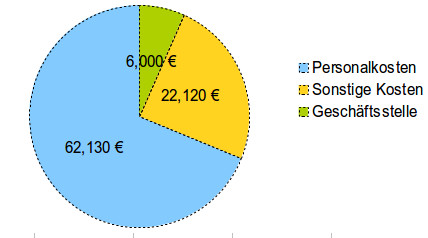
\includegraphics[width=5cm]{pics/kostenarten.jpg}
 \end{column}
\end{columns}
\begin{itemize}
\item Weiterbetrieb nach Anschubphase erfordert mindestens 2 halbe Stellen (Koordination; Technik)
  \begin{itemize}
  \item 60kEUR+
  \end{itemize}
\end{itemize}
}


\frame{
\frametitle{Modelle für die Zukunft}
\parbox{\textwidth}{
  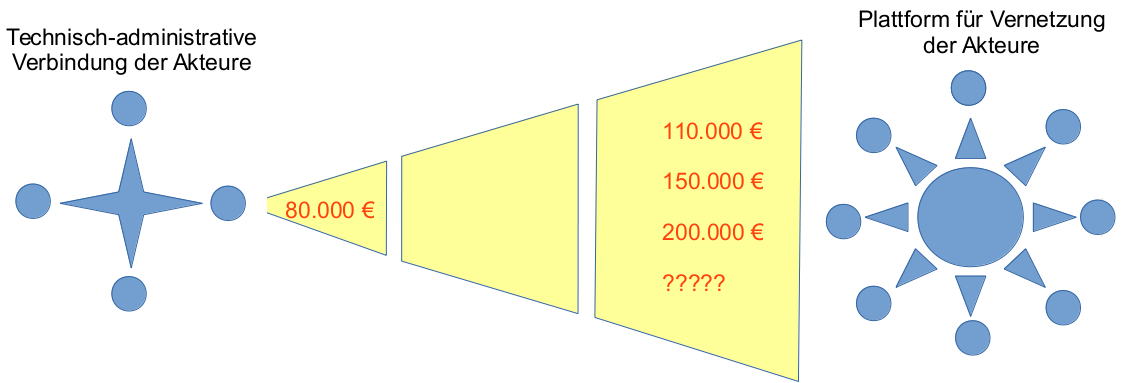
\includegraphics[width=\textwidth]{pics/modelle.png}
}

\begin{tabular}{lr}
Koordination & 
 Unterstützung und Vernetzung\vspace{-.4cm}\\[.1em]
\parbox[t]{.48\textwidth}{
\footnotesize
\begin{itemize}
 \item minimale Koordination
 \item Systemadministration
 \item Support durch Forum
 
 $\to$ kein Wachstum, keine Entwicklung
\end{itemize}
}
&
\footnotesize
\parbox[t]{.48\textwidth}{
\begin{itemize} 
 \item Web 2.0-Funktionen
 \item Benutzerfreundlichkeit
 \item Erweiterung auf entfernte Fachgebiete
 \item breites Leistungsspektrum
 
 $\to$ dauerhafte Entwicklung
\end{itemize}
}
\end{tabular}
}

% \frame{
% \frametitle{Finanzierung für die Zukunft}
% 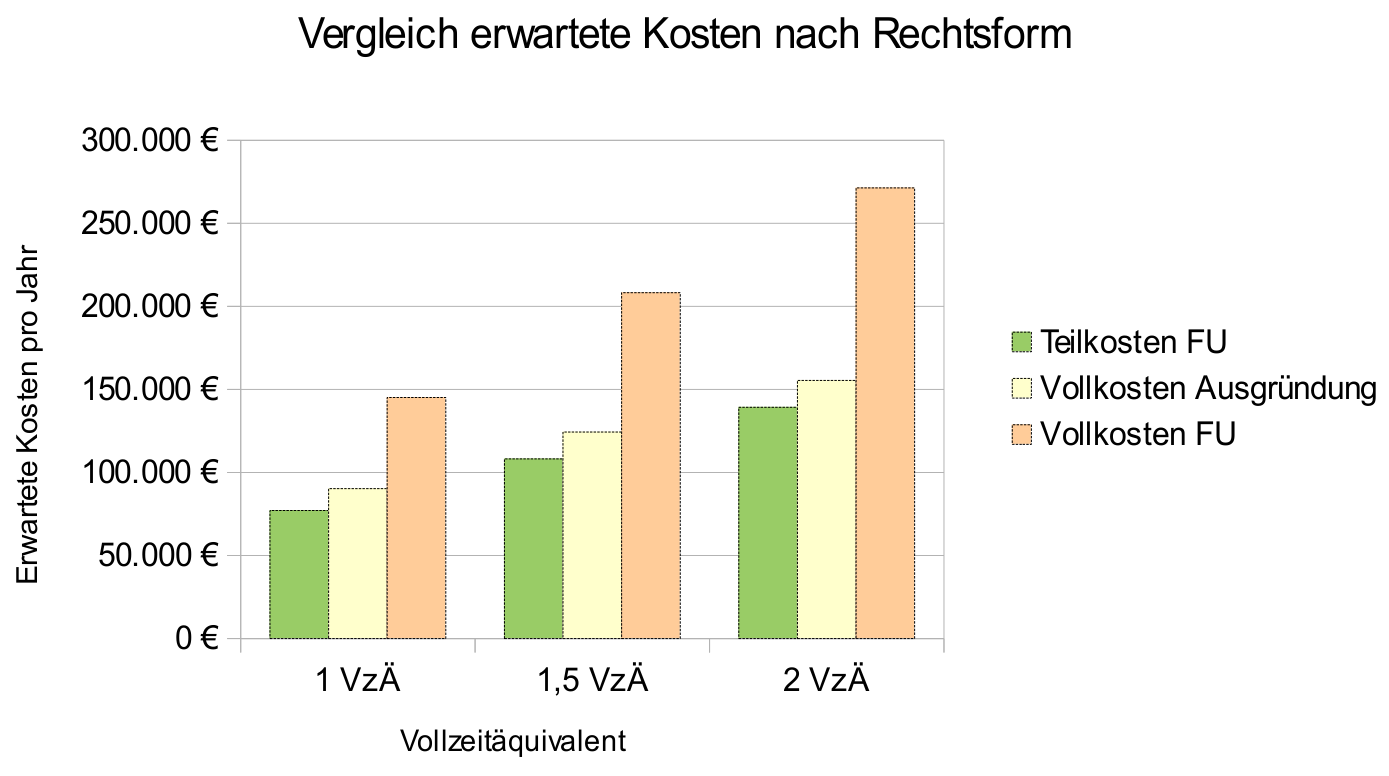
\includegraphics[width=\textwidth]{pics/finanzierung.png}
% }

% 
% \frame{
% \frametitle{Akteure}
% \begin{tabular}{llll}
%  & Leser &  & \\
% Verlag & Bibliotheken&  & Finanzminister\\
%  & Fachgesellschaften &  & DFG\\
%  & Autoren &  & 
% \end{tabular}
% }



% \section{Preise}
% 
% \frame{
% \frametitle{Preisliste für \\Open-Access-Bücher}
% 
% \begin{itemize}
% \item Palgrave Macmillan: 11,000 {\textlira} (17,500 \$)
% % \footnote{
% % \url{http://poynder.blogspot.co.uk/2013/09/de-gruyters-sven-fund-on-state-of-open.html}. 04.03.2014.
% % }
% \item Springer: ca.\, 15,000 \geneuro%\footnote{
% % \url{http://poynder.blogspot.co.uk/2013/09/de-gruyters-sven-fund-on-state-of-open.html}. 04.03.2014.
% % \newline
% % Lustigerweise steht das nicht in der FAQ: \url{http://www.springeropen.com/about/faq/chargesbooks}. 04.03.2014.
% % }
% \item De Gruyter Open: 10.000 {\geneuro} (p.\,M.\ 02/2014)\\
%       (1.500 {\geneuro} bei normalen Büchern, wenn nicht selbst gesetzt)
% \item Brill: 5.000 {\geneuro}
% \end{itemize}
% 
% }
% 
% 
% \frame{
% \frametitle{Geldströme in der geisteswissenschaftlichen Publikationslandschaft}
% 
% 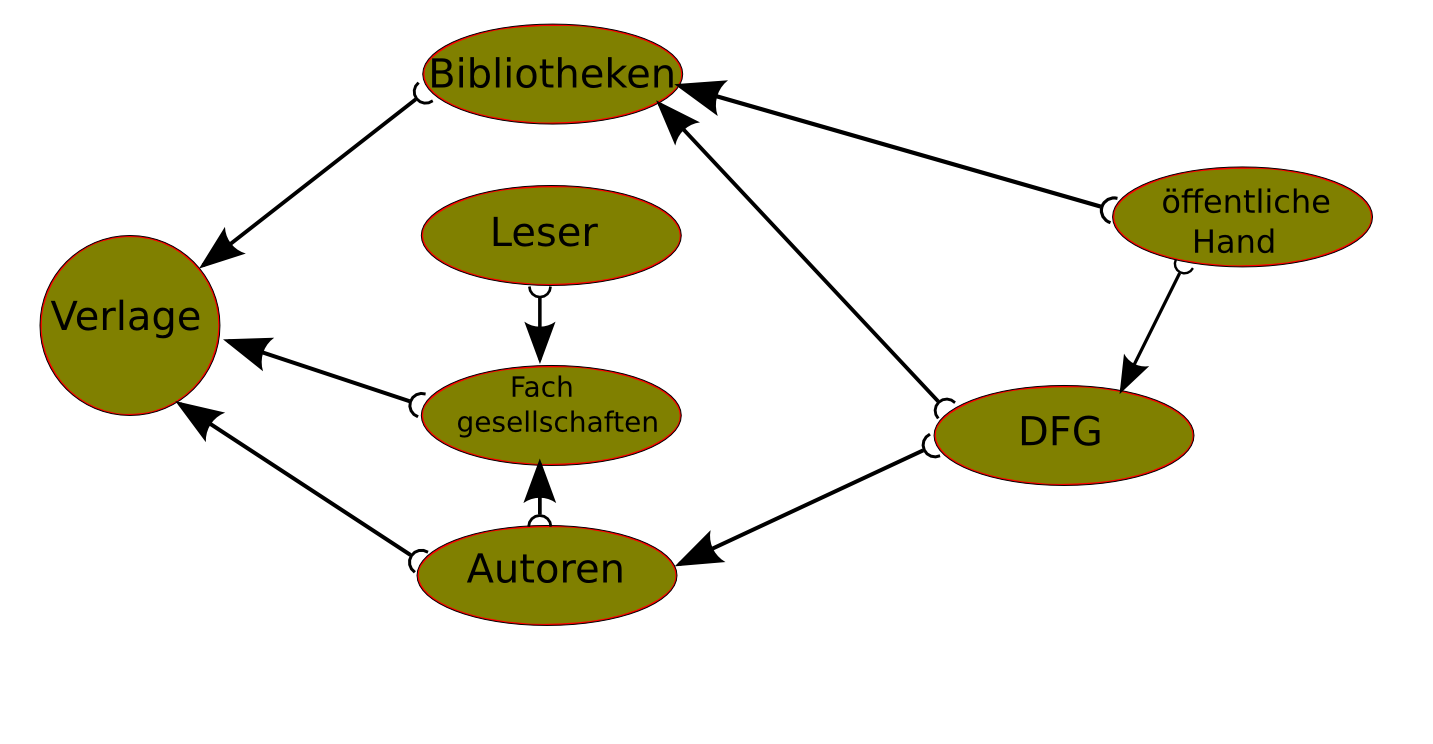
\includegraphics[height=\textheight]{pics/geldstroeme_OA.png}
% 
% }
% 

\section{Annotation}

\frame{ 
\frametitle{Konversion nach XML}

  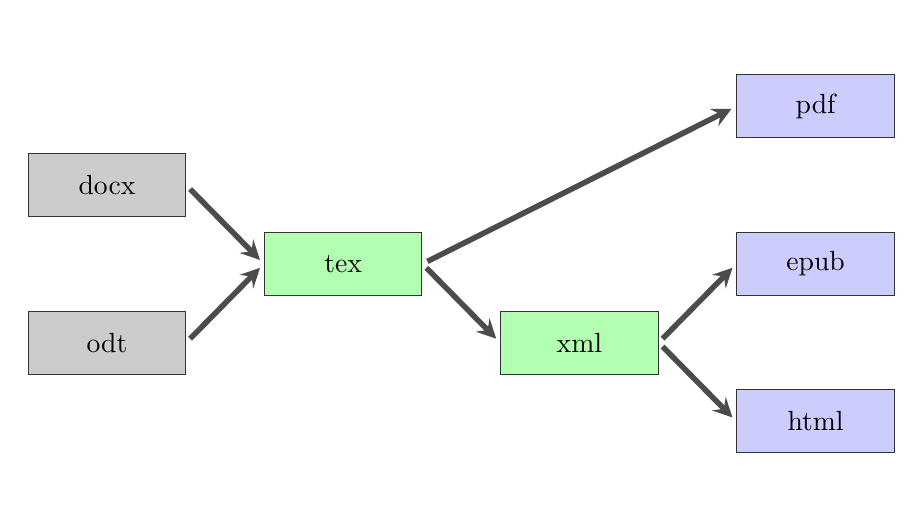
\begin{tikzpicture}
    \tikzstyle{every node}+=[draw=black!80,fill=none,minimum height=8mm,minimum width=20mm]
    \tikzstyle{input}+=[draw,fill=black!20!white]
    \tikzstyle{master}+=[fill=green!30!white]
    \tikzstyle{output}+=[fill=blue!20!white]
    \tikzstyle{tarr}=[-stealth,black!70!white,line width=2pt,shorten >=2pt,shorten <=2pt]

    \node [input]  (odt) at (-4,-1) { odt };
    \node [input]  (docx) at (-4,1) { docx };
    \node [master] (tex) at (-1,0) { tex };
    \node [master] (xml) at (2,-1) { xml };
    \node [output] (pdf) at (5,2) { pdf };
    \node [output] (epub) at (5,0) { epub };
    \node [output] (html) at (5,-2) { html };

    \draw [tarr] (odt.east) -- (tex.west);
    \draw [tarr] (docx.east) -- (tex.west);
    \draw [tarr] (tex.east) -- (xml.west);
    \draw [tarr] (tex.east) -- (pdf.west);
    \draw [tarr] (xml.east) -- (epub.west);
    \draw [tarr] (xml.east) -- (html.west);

    \draw [step=10mm,draw=none] (-5,-3) grid (6,3);

  \end{tikzpicture}
}


\frame{ 
\frametitle{Linguistic Linked Open Data Cloud}
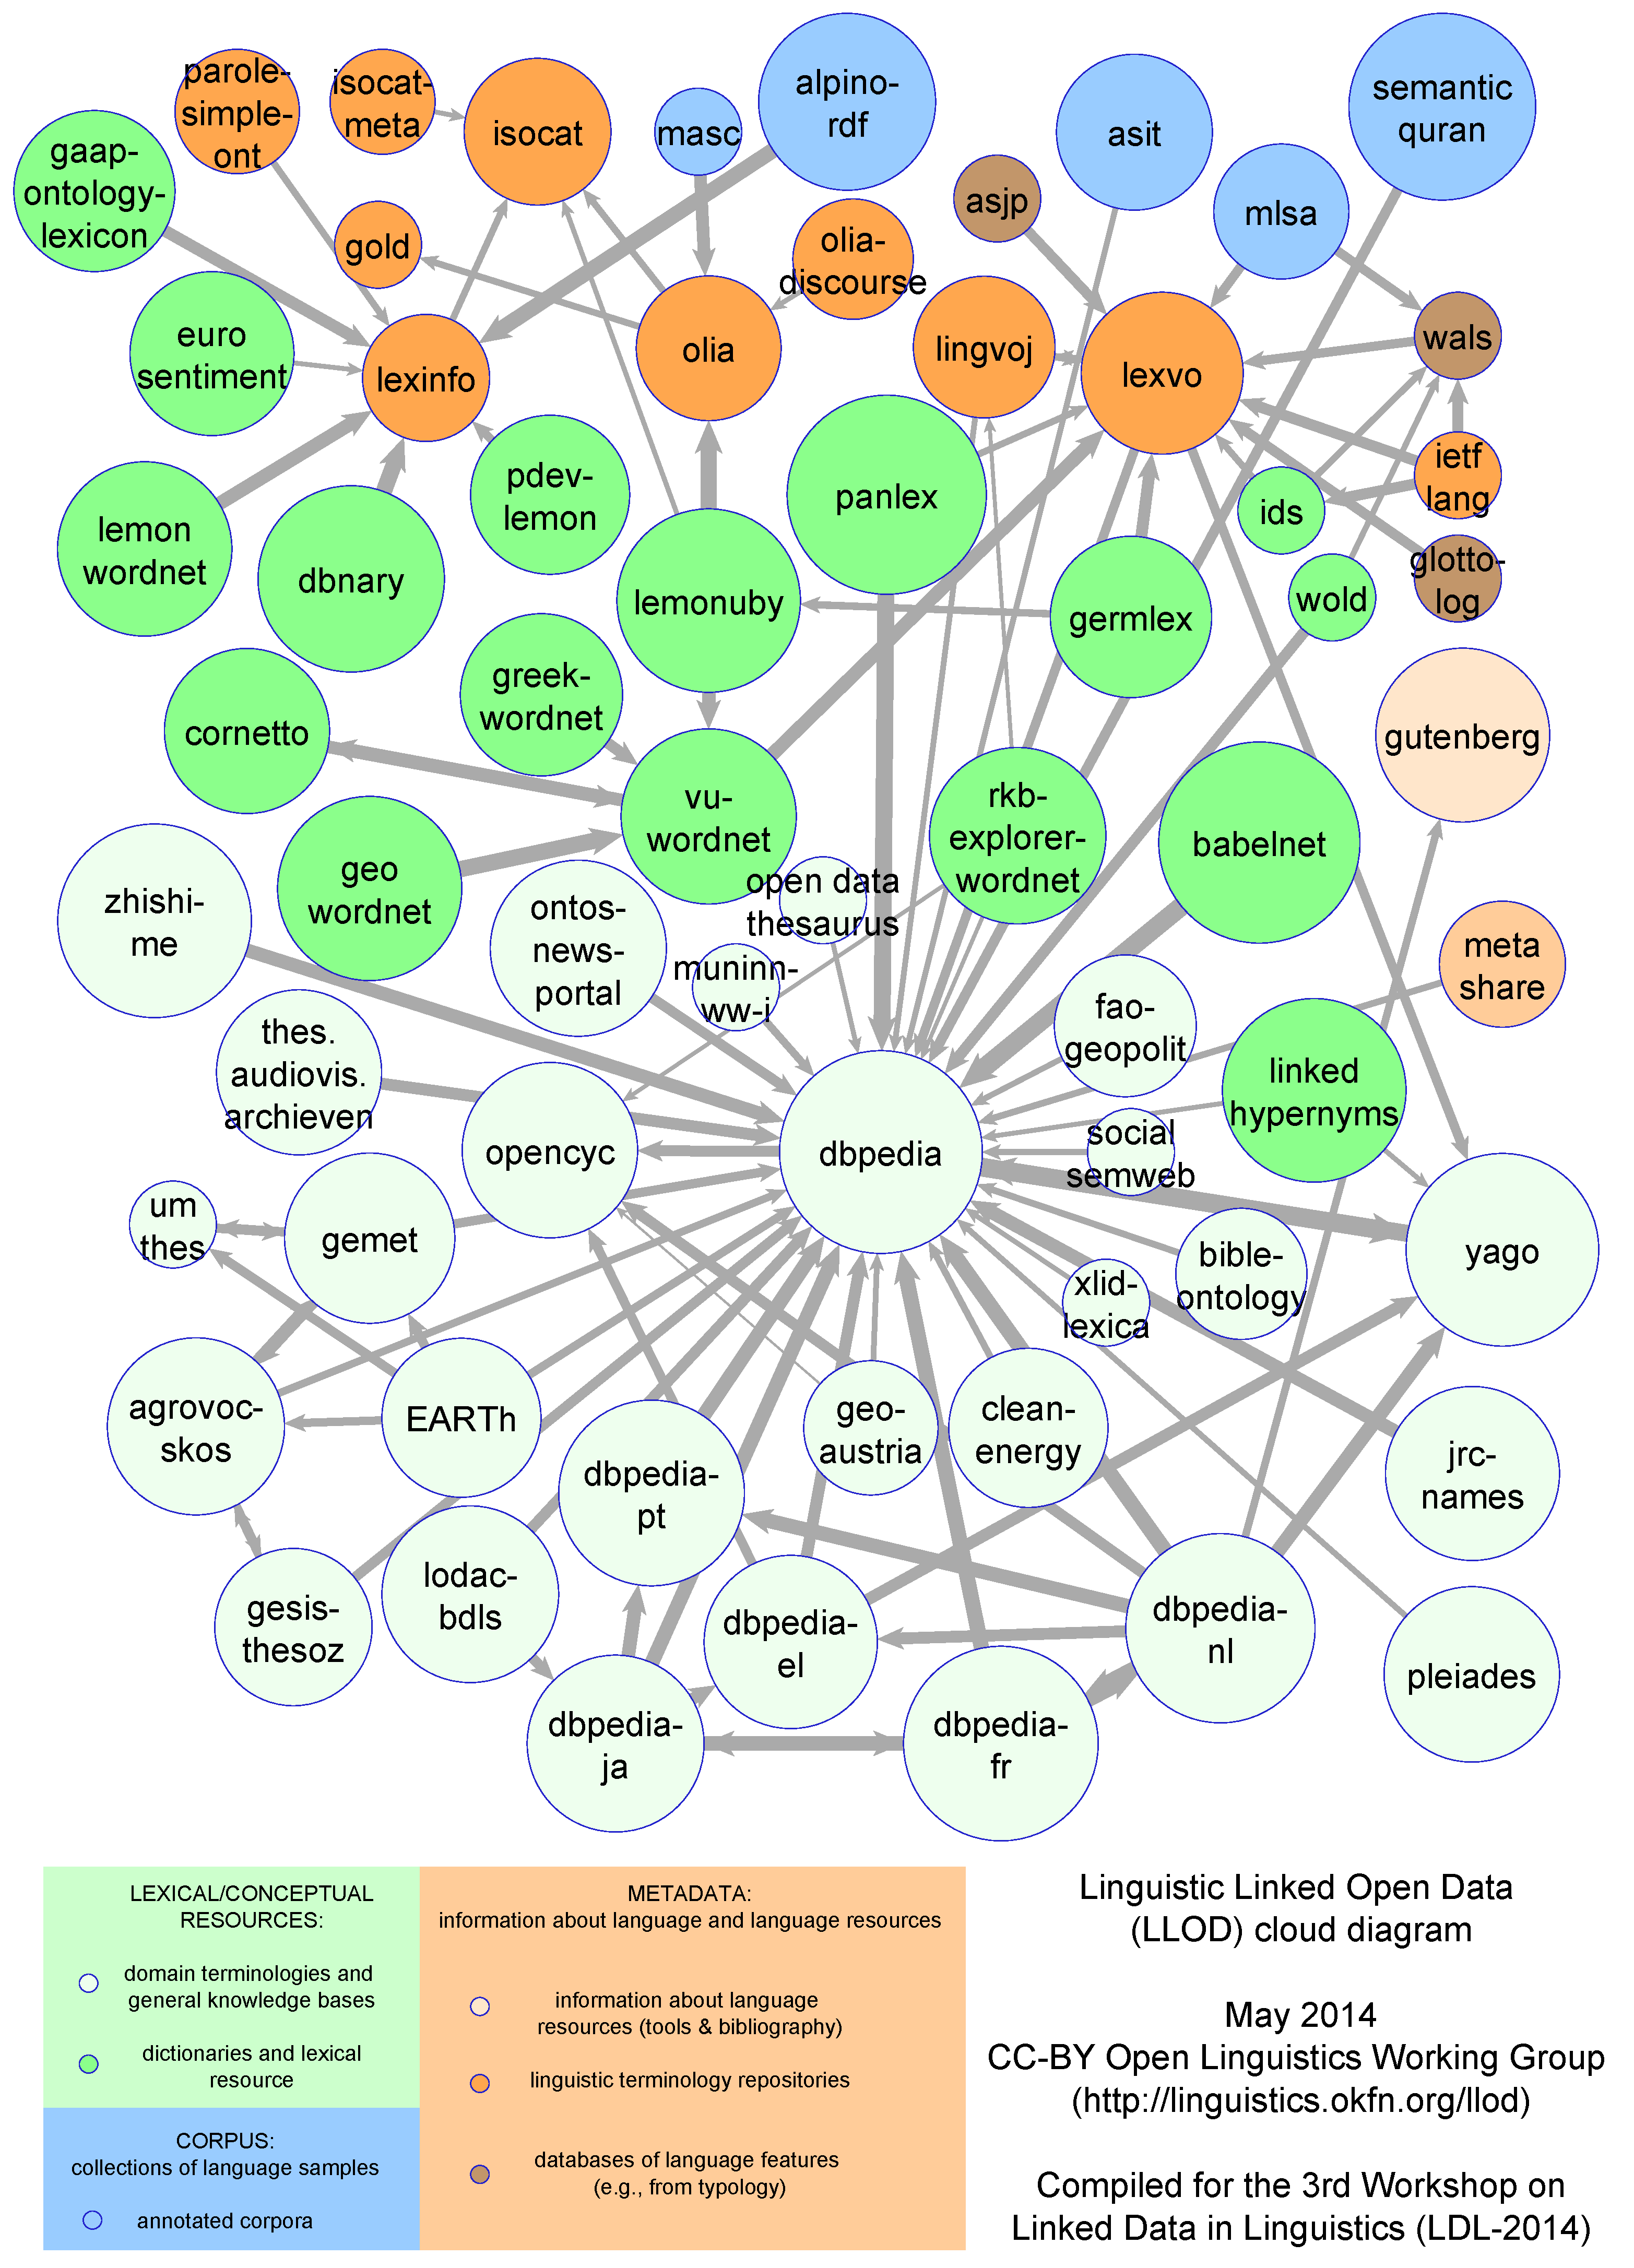
\includegraphics[height=1.5\textheight]{pics/llod.pdf}
}

\frame{ 
\frametitle{Auszeichnung von Beispielen}
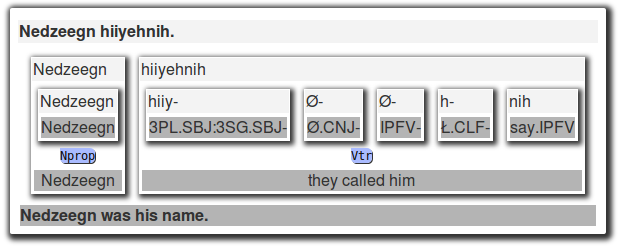
\includegraphics[width=\textwidth]{pics/imt.png}
}

\frame{
\frametitle{Bäume}
\begin{forest}
[VP
[DP[John]]
[V’
[V[sent]]
[DP[Mary]]
[DP[D[a]][NP[letter]]]
]
]
\end{forest}
}

\frame{ 
\frametitle{Merkmal-Wert-Matritzen}
\begin{avm}
\[phon   & \< {\it porcupine\/} \>\\
  feat-a & \@{10} \[feat-aa & type-aa\\
                    feat-ab & \< \[ synsem|loc|cat|head & type-aba\\
                                    feat-abc \tpv{type-abc} 
                                  \],
                                  \textup{NP} \>\\
                    \tp{type-a}
                  \]\\
 feat-b & \@{10} type-b\\ 
 \tp{some-type}
\]
\end{avm}

\begin{itemize}
 \item Verbindung mit Bäumen 
 \item Möglichkeit von js-Visualisierungen
\end{itemize}
}


\frame{ 
\frametitle{Open Review}
\begin{itemize}
 \item In der Konzipierungsphase 
  \item eindeutige Adressierbarkeit von Versionen
  \item in dieser Hinsicht eine spezielle Art von Annotation
\end{itemize}

}

\section{Schluss}

\frame{ 
\frametitle{Noch kein Unterstützer?}
\url{http://langsci-press.org/Meta/sign/}

\includegraphics[height=.7\textheight]{pics/sign.png}
}
\end{document}